The benefits of C integration are numerous: The major computer operating systems are written in C,\cite{Linux, Darwin, WindowsKernel} the C runtime is ubiquitous and generally doesn't conflict with other language runtimes, and C is conducive to high performance programming.

Language designers and maintainers commonly provide support and documentation for how to integrate C modules into projects based in their languages.  Of the top ten most popular languages by pull request on Github,\cite{Octoverse} nine have native support for calling C code\cite{JavascriptCiface, PythonCiface, JavaCiface, RubyCiface, PHPCiface, DotNetCiface, GoCiface, CPPCIface} (the exception, CSS; C, in tenth place, obviously links with itself).

\begin{figure}[htbp!]
        \centering
        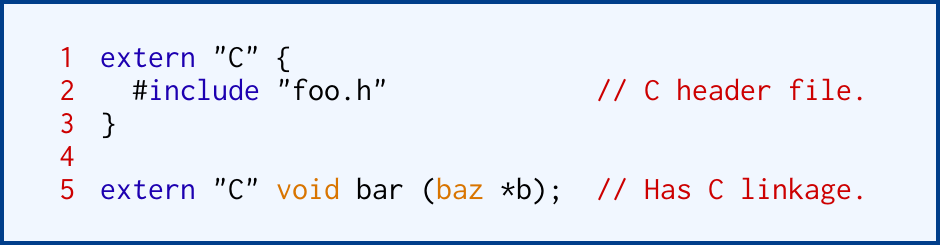
\includegraphics[scale=0.25]{gfx/extern}
        \caption{Example of C++ code that imports a header file from C and exports a function that can be used by a C module.}
        \label{fig:extern-example}
\end{figure}

Fig.~\ref{fig:extern-example} demonstrates that C++ goes to lengths to be compatible with C in both directions.  By using \texttt{extern \textquotedbl{}C\textquotedbl{}}, a symbol can be declared with C linkage, and since all of the native C types correspond to native types in C++, calling back-and-forth between languages is easy.  It means that C++ is compatible with any language with C hooks.  This is the only language we are aware of that has this degree of integration.

Both directions are integral to the design of DEF.  Even though many elements of DEF's syntax are inspired by C, it isn't interchangeable even in simple cases, as C++ is.  Nevertheless, \textit{well-behaved} C header files can be imported directly into DEF.  A header is well-behaved if, as included in a C source file, it satisfies the C parser in itself -- neither expecting tokens prior to beginning, nor requiring tokens after.  Because headers are typically written as interface files, most are well-behaved including all of the standard libraries.
